\chapter{Введение}							% Заголовок

Необходимость изучения систем, которые случайным образом изменяются с течением времени, постоянно растёт. Математическая модель для описания таких систем основана на понятии стохастического процесса.

\section*{Объекты и предмет исследования}
Объектом исследования этой работы являются оценки параметров нелинейных нестационарных процессов в форме суммы двух процессов Леви. Следует отметить, что результаты этих исследований могут иметь прикладную значимость и для более широкого класса моделей.

Предметом исследования являются стохастические связи между оценками параметров модели этих процессов в предположении, что эти оценки получены с помощью различных методов интервального и точечного оценивания.

\subsection*{Случайные процессы}

Для рассуждений о предмете и объекте приведённых исследований, следует привести ряд определений, которые используются далее по тексту.

\begin{define}
	Величина $X$ называется \emph{случайной величиной}, если для каждого данного значения $c$ может быть получена определённая вероятность того, что $X$ не превосходит $c$.
\end{define}

\begin{define}
	$F$ называется \emph{функцией распределения случайной величины} $X$, если для любого $x \in \exR$ выполняется $F(x) = \P\{\, X \leqslant x \,\}$.
\end{define}

\emph{Стохастический (случайный) процесс} рассматривается как множество $\{\, X(t) \mid t \in T \,\}$ случайных величин $X(t)$, определённых на одном вероятностном пространстве, где $T \subset \R$. $T$ может интерпретироваться как время.
\begin{define}
	Случайный процесс называется \emph{дискретным во времени}, если $T \subset \Z$.
\end{define}
\begin{define}
 	Если все случайные величины $X(t)$ принимают значения из фиксированного множества $\J$, то $\J$ называется \emph{пространством состояний} процесса.
\end{define}
Для каждого $t \in T$ функция распределения $X_t$ обозначается $F_t$.
\begin{define}
	Процесс $\{\, X(t) \mid t \in T \,\}$ называется \emph{марковским}, если для каждого конечного подмножества $\{\, t_1, t_2, \ldots, t_n \,\} \subset T$ и $\forall t \in T$ таких, что $t_1 < t_2 < \cdots < t_n < t$, справедливо
\[
\P\{\, X_t \leqslant x \mid X_{t_1} = x_1, X_{t_2} = x_2, \ldots, X_{t_n} = x_n \,\} = \P\{\, X_t \leqslant x \mid X_{t_n} = x_n \,\}.
\]
\end{define}

\subsection*{Стохастические связи между случайными величинами}

\begin{define}
\emph{Стохастическая связь} --- вероятностная зависимость между величинами, которая проявляется только в массе наблюдений.
\end{define}

Для изучения таких связей необходимо наличие достаточно большого количества наблюдений исследуемых величин.

\subsection*{Входные данные и цель работы}

Входными данными являются результаты вычислительных экспериментов по интервальному оцениванию (Сидоровская, 2015 г.) в количестве порядка $10^6$.

Цель работы состоит в том, чтобы оценить стохастические связи между модельными значениями параметров и предоставленными результатами алгоритма интервального оценивания. Это позволит провести исследование качества этого алгоритма.

\section*{Традиционные оценки стохастических связей}
\subsection*{Коэффициент корреляции}

\begin{define}
\emph{Линейным коэффициентом корреляции} вектора случайных величин $\trans{(X, Y)}$ с ненулевыми конечными дисперсиями называется величина
\begin{equation}
	\rho(X, Y) = \frac{\cov(X, Y)}{\sqrt{\D(X)\D(Y)}},
\end{equation}
где $\cov(X, Y) = \E(XY) - \E(X)\E(Y)$ --- ковариация $\trans{(X, Y)}$, а $\D(X)$ и $\D(Y)$ --- соответствующие дисперсии.
\end{define}

Если имеются выборки $\{\, x_i \,\}_{i=1}^n, \{\, y_i \,\}_{i=1}^n$ значений случайных величин $X, Y$, то линейный коэффициент корреляции можно оценить величиной
\begin{equation}
r_{X, Y} = \frac{\sum_{i=1}^{n} (x_i - \overline{x})(y_i - \overline{y})}{\sqrt{\sum_{i=1}^{n} (x_i - \overline{x})^2 \sum_{i=1}^{n} (y_i - \overline{y})^2}}.
\end{equation}

Величины $\rho(X, Y)$, $r_{X, Y}$ инвариантны относительно строго возрастающих линейных преобразований $X, Y$, то есть
\[
\forall a > 0, c > 0, b, d \in \R \colon \rho(X, Y) = \rho(aX + b, cY + d).
\]

\subsubsection*{Необходимые условия применения}
Для вычисления $\rho(X, Y)$ должны существовать ковариация и конечные ненулевые дисперсии величин $X, Y$. При вычислении $r_{X, Y}$ необходимо учитывать, что это не робастная статистика, и убедиться, что выборки не содержат выбросов.
\subsubsection*{Семантика оценки}
Из определения ясно, что $\rho(X, Y) \in [-1, 1]$. Так как это мера линейной зависимости, то выполняется
\[
Y = aX + b, a \neq 0, b \in \R \iff |\rho(X, Y)| = 1.
\]

Если $|\rho(X, Y)| < 1$, то положительный $\rho(X, Y)$ показывает, что значения $X$ и $Y$ имеют тенденцию быть одновременно больше или одновременно меньше соответствующих им средних. Отрицательный --- что значения $X$ и $Y$ имеют тенденцию лежать по разные стороны от соответствующих им средних.

Если случайные величины независимы, то их линейный коэффициент корреляции равен нулю (они называются \emph{некоррелированными}). Обратное, вообще говоря, неверно. Существуют зависимые некоррелированные величины, поэтому невозможно судить о независимости случайных величин $X, Y$, даже если $\rho(X, Y) = 0$.

Тот факт, что коэффициент $\rho$ инвариантен только относительно строго возрастающих \emph{линейных} преобразований, указывает на его узкую применимость. Это ясно из теорем Скляра (\ref{thm:sklar}) и \ref{thm:copula_invariant}, демонстрирующих, что связь между двумя величинами, выражаемая копулой, инвариантна относительно любых строго возрастающих преобразований.

\subsection*{Оценка $\tau$ Кендалла}

\begin{define}
\emph{Коэффициентом ранговой корреляции} вектора случайных величин $\trans{(X, Y)}$ называется величина
\begin{equation}\label{eq:tau}
	\tau(X, Y) = \P\{\, (X - \widetilde{X})(Y - \widetilde{Y}) > 0 \,\} - \P\{\, (X - \widetilde{X})(Y - \widetilde{Y}) < 0 \,\},
\end{equation}
где $\trans{(\widetilde{X}, \widetilde{Y})}$ --- независимая копия $\trans{(X, Y)}$.
\end{define}

Если имеются выборки $\{\, x_i \,\}_{i=1}^n, \{\, y_i \,\}_{i=1}^n$ значений случайных величин $X, Y$, то пары $(x_i, y_i), (x_j, y_j)$, образуемые соответствующими значениями из этих выборок, называются
\begin{itemize}
	\item согласованными, если $(x_i > x_j \text{ и } y_i > y_j) \text{ или } (x_i < x_j \text{ и } y_i < y_j)$;
	\item несогласованными, если $(x_i < x_j \text{ и } y_i > y_j) \text{ или } (x_i > x_j \text{ и } y_i < y_j)$;
\end{itemize}
Если $x_i = x_j \text{ или } y_i = y_j$, то такая пара не классифицируется. Таким образом, коэффициент ранговой корреляции можно оценить величиной
\begin{equation}
\tau_{X, Y} = \frac{(\text{число согласованных пар}) - (\text{число несогласованных пар})}{\frac{1}{2}n(n - 1)}.
\end{equation}

Величины $\tau(X, Y)$, $\tau_{X, Y}$ инвариантны относительно \emph{любых} строго возрастающих линейных преобразований $X, Y$.

\subsubsection*{Необходимые условия применения}
В отличие от линейного коэффициента корреляции коэффициент $\tau$ намного меньше подвержен влиянию выбросов, находящихся в выборке.
\subsubsection*{Семантика оценки}
Из определения ясно, что $\tau_{X, Y} \in [-1, 1]$. Если все пары согласованы, то оценка принимает значение $1$. Если все пары не согласованы, то значение равно $-1$. В случае, когда $X$ и $Y$ независимы, можно ожидать, что оценка будет примерно равна нулю.

Положительный $\tau_{X, Y}$ показывает, что большее количество пар согласовано, а отрицательный~--- что большее количество пар не согласовано.

\section*{Копулы}

\subsection*{Вспомогательные понятия}

Обозначим за $\exR$ расширенную действительную прямую $[-\infty, \infty]$. Прямоугольником $B$ в $\exR^2$ назовём произведение двух отрезков $B = [x_1, x_2] \times [y_1, y_2]$. Единичный квадрат $I^2$ это произведение $I \times I$, где $I = [0, 1]$. Двуместной действительной функцией назовём функцию $H$, область определения ($\Dom{H}$) которой есть подмножество $\exR^2$, а множество значений ($\Ran{H}$) --- подмножество $\R$.

\begin{define}
	Пусть $S_1, S_2$ --- непустые подмножества $\exR$, а $H$ --- такая двуместная действительная функция, что $\Dom{H} = S_1 \times S_2$. Пусть $B = [x_1, x_2] \times [y_1, y_2]$ --- прямоугольник, все вершины которого лежат в $\Dom{H}$. Тогда \emph{$H$-объёмом} $B$ называется
\[
V_H(B) = \Diff_{y_1}^{y_2}\Diff_{x_1}^{x_2}H(x, y).
\]
\end{define}

\begin{define}
	Двуместная действительная функция $H$ называется \emph{2-возрастающей}, если $V_H(B) \geqslant 0$ для всех прямоугольников $B$, чьи вершины лежат в $\Dom{H}$.
\end{define}

2-возрастание, вообще говоря, не связано с возрастанием по аргументам, но справедлива следующая лемма.

\begin{lemma}
	Пусть $S_1, S_2$ --- непустые подмножества $\exR$, а $H$ --- 2-возрастающая функция с $\Dom{H} = S_1 \times S_2$. Пусть $x_1, x_2 \in S_1$ такие, что $x_1 \leqslant x_2$, и $y_1, y_2 \in S_2$ такие, что $y_1 \leqslant y_2$. Тогда функция $t \mapsto H(t, y_2) - H(t, y_1)$ не убывает на $S_1$, а $t \mapsto H(x_2, t) - H(x_1, t)$ не убывает на $S_2$.
\end{lemma}

Из этой леммы ясно, что с дополнительным предположением 2-возрастающая функция будет неубывающей по каждому аргументу.

\begin{define}
	Функция $H \colon S_1 \times S_2 \to \R$ называется \emph{заземлённой}, если
\[
H(x, a_2) = 0 = H(a_1, y), \forall (x, y) \in S_1 \times S_2,
\]
где $a_1, a_2$ --- наименьшие элементы $S_1, S_2$ соответственно.
\end{define}

\begin{lemma}
	Пусть $S_1, S_2$ --- непустые подмножества $\exR$, а $H$ --- заземлённая 2-возрастающая функция с $\Dom{H} = S_1 \times S_2$. Тогда функция $H(x, y)$ не убывает по каждому аргументу.
\end{lemma}

\begin{define}
	Если множества $S_1, S_2$ имеют наибольшие элементы $b_1, b_2$ соответственно, то $H \colon S_1 \times S_2 \to \R$ имеет \emph{маргиналы} $F$ и $G$:
	\begin{gather}
		\Dom{F} = S_1, F(x) = H(x, b_2) \\
		\Dom{G} = S_2, G(y) = H(b_1, y)
	\end{gather}
\end{define}

\begin{lemma}\label{lm:precont}
	Пусть $S_1, S_2$ --- непустые подмножества $\exR$, а $H$ --- заземлённая 2-возрастающая функция с маргиналами и $\Dom{H} = S_1 \times S_2$. Пусть $(x_1, y_1), (x_2, y_2)$ --- любые точки из $S_1 \times S_2$, тогда
\[
|H(x_2, y_2) - H(x_1, y_1)| \leqslant |F(x_2) - F(x_1)| + |G(y_2) - G(y_1)|.
\]
\end{lemma}

\subsection*{Субкопулы и копулы}

Принимая во внимание введённые понятия, можно определить копулы. Но перед этим определяются субкопулы\cite{Nelsen1999}.

\begin{define}
	\emph{Двумерной субкопулой} называется функция $C'$, удовлетворяющая следующим свойствам:
	\begin{enumerate}
	\item $\Dom{C'} = S_1 \times S_2$, где $S_1, S_2$ --- подмножества $I$, содержащие $0$ и $1$;
	\item $C'$ --- заземлённая и 2-возрастающая;
	\item Для каждого $u \in S_1$ и каждого $v \in S_2$:
		\begin{gather}
			C'(u, 1) = u \\
			C'(1, v) = v.
		\end{gather}
	\end{enumerate}
\end{define}

Из данного определения ясно, что $\Ran{C'} \subset I$.

\begin{define}
	\emph{Двумерной копулой} называется двумерная субкопула $C$ с областью определения $I^2$.
\end{define}

Многие важные свойства копул на самом деле принадлежат субкопулам. Но именно копулы имеют важные приложения в теории вероятностей и статистике.

\begin{theorem}\label{thm:bounds}
	Пусть $C'$ --- субкопула, тогда $\forall (u, v) \in \Dom{C'}$
	\begin{equation}\label{eq:bounds}
		\max (u + v - 1, 0) \leqslant C'(u, v) \leqslant \min (u, v).
	\end{equation}
\end{theorem}

Теорема \ref{thm:bounds} справедлива и для копул, потому что любая копула является субкопулой. Границы в неравенстве \eqref{eq:bounds} сами являются копулами, обозначаемыми $W(u, v) = \max (u + v - 1, 0)$ и $M(u, v) = \min (u, v)$. Ещё одна часто встречающаяся копула $\Pi(u, v) = uv$.

Следующая теорема является прямым следствием леммы \ref{lm:precont} и демонстрирует равномерную непрерывность субкопул, а значит и копул, в $I^2$.

\begin{theorem}\label{thm:cont}
	Пусть $C'$ --- субкопула, тогда для любых $(u_1, v_1), (u_2, v_2) \in \Dom{C'}$
\[
|C'(u_2, v_2) - C'(u_1, v_1)| \leqslant |u_2 - u_1| + |v_2 - v_1|.
\]
\end{theorem}

Следующее определение вводит понятие сечений копул, которые используются при построении копул и интерпретации их характеристик.

\begin{define}
	Пусть $C$ --- копула, $a$ --- любое число из $I$. Тогда \emph{горизонтальным сечением} $C$ называется функция из $I$ в $I$, соответствующая $t \mapsto C(t, a)$; \emph{вертикальным сечением} $C$ называется функция из $I$ в $I$, соответствующая $t \mapsto C(a, t)$; \emph{диагональным сечением} $C$ называется функция из $I$ в $I$, соответствующая $t \mapsto C(t, t)$.
\end{define}

Так как копулы равномерно непрерывны на своей области определения и не убывают по каждому аргументу, то справедлива следующая теорема.

\begin{theorem}\label{thm:sections}
	Горизонтальные, вертикальные и диагональные сечения копул не убывают и равномерно непрерывны на $I$.
\end{theorem}

Из теоремы \ref{thm:cont} следует, что график любой копулы $z = C(u, v)$ есть непрерывная поверхность, лежащая в единичном кубе $I^3$ и проходящая через точки $(0, 0, 0), (0, 1, 0), (1, 0, 0), (1, 1, 1)$. Из теоремы \ref{thm:bounds} следует, что график лежит между поверхностями $z = W(u, v)$ и $z = M(u, v)$.

\begin{figure}[H]
	\centering
	\begin{subfigure}{.5\textwidth}
		\centering
		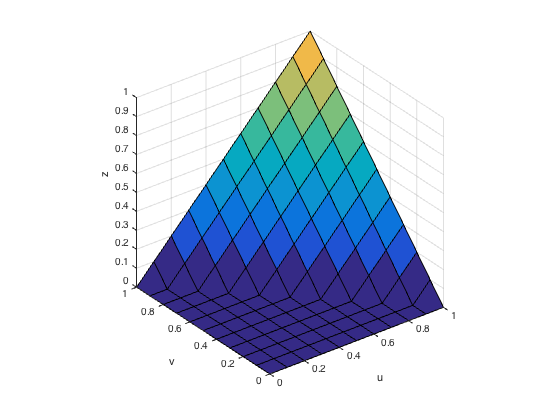
\includegraphics[width=\linewidth]{W.png}
		\caption{$z = W(u, v)$}
	\end{subfigure}%
	\begin{subfigure}{.5\textwidth}
		\centering
		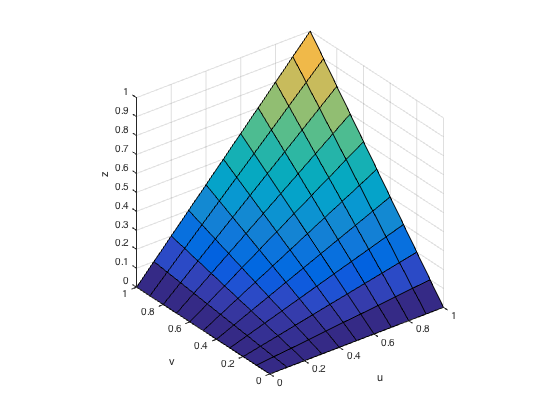
\includegraphics[width=\linewidth]{P.png}
		\caption{$z = P(u, v)$}
	\end{subfigure}
	\begin{subfigure}{.5\textwidth}
		\centering
		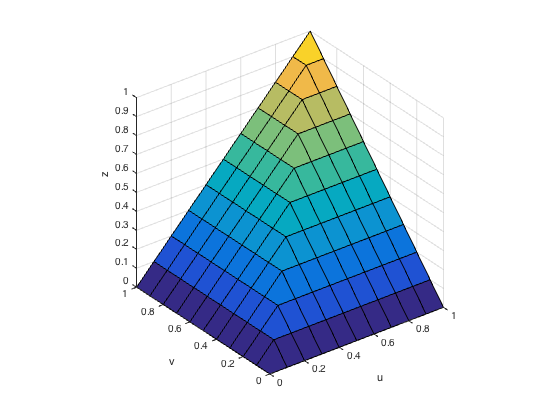
\includegraphics[width=\linewidth]{M.png}
		\caption{$z = M(u, v)$}
	\end{subfigure}
	\caption{Графики копул $W$, $P$ и $M$}
\end{figure}

Можно изображать копулы проще, используя \emph{контурные диаграммы}, то есть изображая его \emph{множества уровней} $\{\, (u, v) \in I^2 \mid C(u, v) = \text{константа} \,\}$. В общем случае требуется помечать, какое множество относится к какому значению константы $t$, но из-за свойств копулы соответствующее множество всегда содержит точки $(1, t), (t, 1)$, так как $C(1, t) = t = C(t, 1)$.

\begin{figure}[H]
	\centering
	\begin{subfigure}{.3\textwidth}
		\centering
		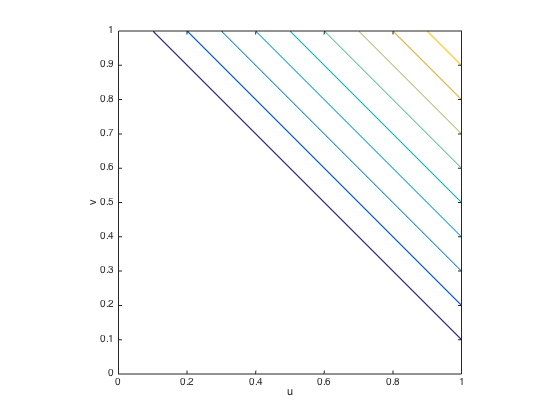
\includegraphics[width=\linewidth]{CW.png}
		\caption{$W(u, v)$}
	\end{subfigure}%
	\begin{subfigure}{.3\textwidth}
		\centering
		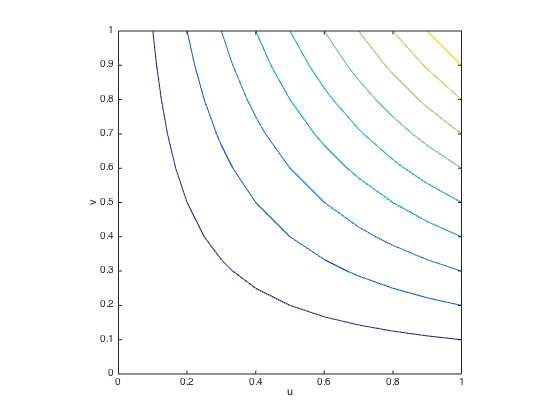
\includegraphics[width=\linewidth]{CP.png}
		\caption{$P(u, v)$}
	\end{subfigure}
	\begin{subfigure}{.3\textwidth}
		\centering
		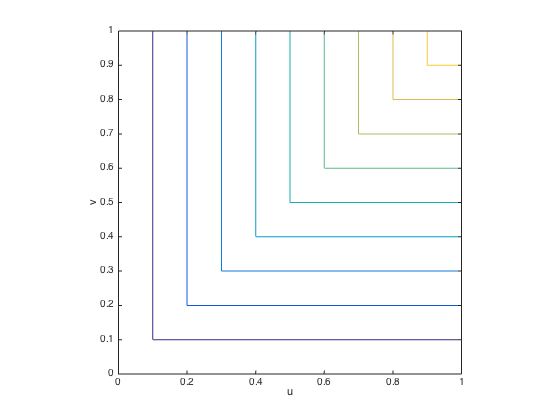
\includegraphics[width=\linewidth]{CM.png}
		\caption{$M(u, v)$}
	\end{subfigure}
	\caption{Контурные диаграммы копул $W$, $P$ и $M$}
\end{figure}

\subsection*{Теорема Скляра}

Из рассмотренного ранее ясно, что при определении копул не привлекаются понятия из теории вероятностей или статистики. Это позволяет без лишней сложности изучать копулы и манипулировать ими, однако наибольшую роль приложения копул играют именно в статистике. Чтобы представить фундамент этих приложений, теорему Скляра, необходимо ввести некоторые стохастические понятия.

\begin{define}
	\emph{Функцией распределения} называется функция $F$ с областью определения $\exR$ такая, что
	\begin{enumerate}
	\item $F$ не убывает;
	\item $F(-\infty) = 0$ и $F(\infty) = 1$.
	\end{enumerate}
\end{define}

\begin{define}
	\emph{Совместной функцией распределения} называется функция $H$ с областью определения $\exR^2$ такая, что
	\begin{enumerate}
	\item $H$ --- 2-возрастающая;
	\item $H(x, -\infty) = H(-\infty, y) = 0$ и $H(\infty, \infty) = 1$.
	\end{enumerate}
\end{define}

Таким образом $H$ заземлена и, так как $\Dom{H} = \exR^2$, имеет маргиналы $F(x) = H(x, \infty)$ и $G(y) = H(\infty, y)$. Учитывая теорему \ref{thm:sections}, ясно, что $F(x)$ и $G(y)$ --- функции распределения.

На самом деле в этих определениях также нет ничего стохастического, например, упоминаний случайных величин. Но все функции распределения, встречающиеся в статистике, удовлетворяют данным определениям, а значит полученные результаты будут справедливы и для них, несмотря на какие-либо дополнительные ограничения.

\begin{theorem}[Теорема Скляра]\label{thm:sklar}
	Пусть $H$ --- совместная функция распределения с маргиналами $F$ и $G$. Тогда существует копула $C$ такая, что для любых $x, y \in \exR$
\begin{equation}\label{eq:sklar}
	H(x, y) = C(F(x), G(y)).
\end{equation}
Если $F$ и $G$ непрерывны, то $C$ единственна; иначе $C$ единственна на $\Ran{F} \times \Ran{G}$.

Обратно, если $C$ --- копула, а $F$ и $G$ --- функции распределения, то $H$, определяемая уравнением \eqref{eq:sklar}, является совместной функцией распределения с маргиналами $F$ и $G$.
\end{theorem}

Уравнение \eqref{eq:sklar} может быть обращено, чтобы выражать копулу через совместную функцию распределения и обратные одномерные функции распределения. Однако, если $F$ и $G$ возрастают нестрого, то они не имеют обратных функций в обычном смысле. Поэтому требуется ввести понятие квазиобратной функции.

\begin{define}
	Пусть $F$ --- функция распределения. Тогда \emph{квазиобратной} к $F$ называется любая функция $F^{(-1)}$ с областью определения $I$ такая, что
	\begin{enumerate}
	\item Если $t \in \Ran{F}$, то $F^{(-1)}(t) = x$, где $x$ --- любое из $\exR$ такое, что $F(x) = t$;
	\item Если $t \notin \Ran{F}$, то
	\[
	F^{(-1)}(t) = inf \{\, x \mid F(x) \geqslant t \,\} = sup \{\, x \mid F(x) \leqslant t \,\}
	\]
	\end{enumerate}
\end{define}
Если $F$ строго возрастает, то существует единственная $F^{(-1)} = F^{-1}$.

\begin{theorem}
	Пусть $H$ --- совместная функция распределения с маргиналами $F$ и $G$, а $C'$ субкопула такая, что
	\begin{enumerate}
	\item $\Dom{C'} = \Ran{F} \times \Ran{G}$;
	\item Для любых $x, y \in \exR$ выполняется $H(x, y) = C'(F(x), G(y))$.
	\end{enumerate}
Тогда $\forall (u, v) \in \Dom{C'}$
\[
C'(u, v) = H(F^{(-1)}(u), G^{(-1)}(v)).
\]
\end{theorem}

Когда $F$ и $G$ непрерывны, то это справедливо и для копул, что позволяет получать копулы из совместных функций распределения.

Полезно заметить, что область определения каждой копулы можно расширить до $\exR^2$ так, чтобы она стала совместной функцией распределения с маргиналами, равномерными на $I$. Если $C$ --- копула, то $H_C$ определяется на $\exR^2$ как
\[
H_C(x, y) =
\begin{cases}
0, &x < 0 \text{ или } y < 0, \\
C(x, y), &(x, y) \in I^2, \\
x, &y > 1, x \in I, \\
y, &x > 1, y \in I, \\
1, &x > 1 \text{ и } y > 1.
\end{cases}
\]

\subsection*{Копулы и случайные величины}

Говорят, что случайная величина непрерывна, если её функция распределения непрерывна. Теперь теорема \ref{thm:sklar} может быть приведена в терминах случайных величин.

\begin{theorem}\label{thm:probsklar}
	Пусть $X, Y$ --- случайные величины с распределениями $F, G$ соответственно, и совместным распределением $H$. Тогда выполняется уравнение \eqref{eq:sklar}.
Если $F$ и $G$ непрерывны, то $C$ единственна; иначе $C$ единственна на $\Ran{F} \times \Ran{G}$.
\end{theorem}

Копула $C$ в теореме \ref{thm:probsklar} называется копулой случайных величин $X, Y$ и обозначается $C_{XY}$. Следующая теорема демонстрирует, что копула $\Pi$ характеризует независимые случайные величины.

\begin{theorem}
	Пусть $X, Y$ --- непрерывные случайные величины. Тогда $X$ и $Y$ независимы тогда и только тогда, когда $C_{XY} = \Pi$.
\end{theorem}

Ещё одним удобным свойством копул является то, что они либо инвариантны, либо предсказуемо меняются относительно строго монотонных преобразований

\begin{theorem}\label{thm:copula_invariant}
	Пусть $X, Y$ --- непрерывные случайные величины c копулой $C_{XY}$. Если $\alpha$ и $\beta$ строго возрастают на $\Ran{X}$ и $\Ran{Y}$ соответственно, то $C_{\alpha(X)\beta(Y)} = C_{XY}$. Таким образом $C_{XY}$ инвариантна относительно строго возрастающих преобразований $X$ и $Y$.
\end{theorem}

\begin{theorem}
	Пусть $X, Y$ --- непрерывные случайные величины c копулой $C_{XY}$. Пусть $\alpha$ и $\beta$ строго монотонны на $\Ran{X}$ и $\Ran{Y}$ соответственно.
	\begin{enumerate}
	\item Если $\alpha$ строго возрастает, а $\beta$ строго убывает, то
	\[
	C_{\alpha(X)\beta(Y)} = u - C_{XY}(u, 1 - v).
	\]
	\item Если $\alpha$ строго убывает, а $\beta$ строго возрастает, то
	\[
	C_{\alpha(X)\beta(Y)} = v - C_{XY}(1 - u, v).
	\]
	\item Если $\alpha$ и $\beta$ строго убывают, то
	\[
	C_{\alpha(X)\beta(Y)} = u + v - 1 + C_{XY}(1 - u, 1 - v).
	\]
	\end{enumerate}
\end{theorem}

\subsection*{Порядок}

\begin{define}
	Если $C_1$ и $C_2$ --- копулы, то говорят, что $C_1$ меньше $C_2$, и пишут $C_1 \prec C_2$, если $C_1(u, v) \leqslant C_2(u, v)$ для всех $u, v \in I$.
\end{define}

Таким образом, $W$ меньше любой другой копулы, а $M$ --- больше. Так заданный порядок является частичным, потому что существуют несравнимые копулы.

\subsection*{Многомерные копулы}

Многие, но не все, результаты, перечисленные выше, могут быть перенесены на случай многомерных копул. Для это требуется вспомогательная нотация. Для любого $n = 1, 2, 3, \ldots$ выражение $\exR^n$ обозначает произведение $n$ множителей $\exR \times \exR \times \cdots \times \exR$. Элементы $\exR^n$ обозначаются $\bm{a} = (a_1, a_2, \ldots, a_n)$, и $\bm{a} \leqslant \bm{b}$ выполняется, если $a_k \leqslant b_k$ для $k = 1, 2, \ldots, n$. Для $\bm{a} \leqslant \bm{b}$ выражение $[\bm{a}, \bm{b}]$ обозначает прямоугольник $B = [a_1, b_1] \times [a_2, b_2] \times \cdots \times [a_n, b_n]$. Единичный $n$-мерный куб $I^n$ и $n$-местная действительная функция определяются аналогично.

\begin{define}
	Пусть $S_1, S_2, \ldots, S_n$ --- непустые подмножества $\exR^n$, а $H$ --- такая $n$-местная действительная функция, что $\Dom{H} = S_1 \times S_2 \times \cdots \times S_n$. Пусть $B = [\bm{a}, \bm{b}]$ --- прямоугольник, все вершины которого лежат в $\Dom{H}$. Тогда \emph{$H$-объёмом} $B$ называется
\[
V_H(B) = \Diff_{\bm{a}}^{\bm{b}}H(\bm{t}) = \Diff_{a_n}^{b_n}\Diff_{a_{n-1}}^{b_{n-1}}\cdots\Diff_{a_1}^{b_1}H(\bm{t}).
\]
\end{define}

\begin{define}
	$n$-местная действительная функция $H$ называется \emph{$n$-возрастающей}, если $V_H(B) \geqslant 0$ для всех прямоугольников $B$, чьи вершины лежат в $\Dom{H}$.
\end{define}

\begin{define}
	Функция $H \colon S_1 \times S_2 \times \cdots \times S_n \to \R$ называется \emph{заземлённой}, если
\[
H(\bm{t}) = 0, \text{ для всех } \bm{t} \in \Dom{H} \text{ таких, что } t_k = a_k \text{ хотя бы для одного } k,
\]
где $a_1, a_2, \ldots, a_n$ --- наименьшие элементы $S_1, S_2, \ldots, S_n$ соответственно.
\end{define}

\begin{define}
	Если множества $S_1, S_2, \ldots, S_n$ имеют наибольшие элементы $b_1, b_2, \ldots, b_n$ соответственно, то $H \colon S_1 \times S_2 \times \cdots \times S_n \to \R$ имеет \emph{маргиналы}, и одномерными маргиналами являются функции:
	\[
		H_k(x) = H(b_1, \ldots, b_{k-1}, x, b_{k+1}, \ldots, b_n) \text{ для всех } x \text{ из } S_k.
	\]
\end{define}

\begin{lemma}
	Пусть $S_1, S_2, \ldots, S_n$ --- непустые подмножества $\exR$, а $H$ --- заземлённая $n$-возрастающая функция с $\Dom{H} = S_1 \times S_2 \times \cdots \times S_n$. Тогда функция $H$ не убывает по каждому аргументу.
\end{lemma}

\begin{lemma}
	Пусть $S_1, S_2, \ldots, S_n$ --- непустые подмножества $\exR$, а $H$ --- заземлённая $n$-возрастающая функция, имеющая маргиналы, и $\Dom{H} = S_1 \times S_2 \times \cdots \times S_n$. Пусть $\bm{x} = (x_1, x_2, \ldots, x_n), \bm{y} = (y_1, y_2, \ldots, y_n)$ --- любые точки из $\Dom{H}$, тогда
\[
|H(\bm{x}) - H(\bm{y})| \leqslant \sum_{k=1}^n|H_k(x_k) - H_k(y_k)|.
\]
\end{lemma}

\begin{define}
	\emph{$n$-мерной субкопулой} называется функция $C'$, удовлетворяющая следующим свойствам:
	\begin{enumerate}
	\item $\Dom{C'} = S_1 \times S_2 \times \cdots \times S_n$, где каждое $S_k$ --- подмножество $I$, содержащее $0$ и $1$;
	\item $C'$ --- заземлённая и $n$-возрастающая;
	\item $C'$ имеет одномерные маргиналы $C'_k, k = 1, 2, \ldots, n$, удовлетворяющие:
	\[
	C'_k(u) = u \text{ для всех } u \in S_k
	\]
	\end{enumerate}
\end{define}

Из данного определения ясно, что $\Ran{C'} \subset I$.

\begin{define}
	\emph{$n$-мерной копулой} называется $n$-мерная субкопула $C$ с областью определения $I^n$.
\end{define}

\begin{theorem}
	Пусть $C'$ --- субкопула, тогда для любых $\bm{u}, \bm{v} \in \Dom{C'}$
\[
|C'(\bm{v}) - C'(\bm{u})| \leqslant \sum_{k=1}^n|v_k - u_k|.
\]
\end{theorem}

\begin{define}
	\emph{$n$-мерной функцией распределения} называется функция $H$ с областью определения $\exR^n$ такая, что
	\begin{enumerate}
	\item $H$ --- $n$-возрастающая;
	\item $H(\bm{t}) = 0, \text{ для всех } \bm{t} \in \exR^n \text{ таких, что } t_k = -\infty \text{ хотя бы для одного } k$ и $H(\infty, \infty, \ldots, \infty) = 1$.
	\end{enumerate}
\end{define}

Таким образом $H$ заземлена и, так как $\Dom{H} = \exR^n$, имеет одномерные маргиналы $F_1, F_2, \ldots, F_n$, являющиеся функциями распределения.

\begin{theorem}[Теорема Скляра для $n$ измерений]\label{thm:nsklar}
	Пусть $H$ --- $n$-мерная функция распределения с маргиналами $F_1, F_2, \ldots, F_n$. Тогда существует $n$-мерная копула $C$ такая, что для любого $\bm{x} \in \exR^n$
\begin{equation}\label{eq:nsklar}
	H(\bm{x}) = C(F_1(x_1), F_2(x_2), \ldots, F_n(x_n)).
\end{equation}
Если $F_1, F_2, \ldots, F_n$ непрерывны, то $C$ единственна; иначе $C$ единственна на $\Ran{F_1} \times \Ran{F_2} \times \cdots \times \Ran{F_n}$.

Обратно, если $C$ --- копула, а $F_1, F_2, \ldots, F_n$ --- функции распределения, то $H$, определяемая уравнением \eqref{eq:nsklar}, является $n$-мерной функцией распределения с маргиналами $F_1, F_2, \ldots, F_n$.
\end{theorem}

\begin{theorem}
	Пусть $H, F_1, F_2, \ldots, F_n$ и $C$ такие же, как в теореме \ref{thm:nsklar}. Тогда $\forall \bm{u} \in I^n$
\[
C(\bm{u}) = H(F_1^{(-1)}(u_1), F_2^{(-1)}(u_2), \ldots, F_n^{(-1)}(u_n)).
\]
\end{theorem}

Расширения копул $W, \Pi, M$ на $n$ измерений обозначаются $W^n, \Pi^n, M^n$ соответственно и выражаются как
\begin{gather}
	W^n(\bm{u}) = \max (u_1 + u_2 + \cdots + u_n - n + 1, 0) \\
	\Pi^n(\bm{u}) = u_1 u_2 \cdots u_n \\
	M^n(\bm{u}) = \min (u_1, u_2, \ldots, u_n)
\end{gather}
Функции $\Pi^n, M^n$ являются копулами для всех $n = 2, 3, \ldots$, однако $W^n$ --- не копула для любых $n > 2$. Несмотря на это, существует аналог теоремы \ref{thm:bounds}.

\begin{theorem}\label{thm:nbounds}
	Пусть $C'$ --- $n$-мерная субкопула, тогда $\forall \bm{u} \in \Dom{C'}$
	\begin{equation}\label{eq:nbounds}
		W^n(\bm{u}) \leqslant C'(\bm{u}) \leqslant M^n(\bm{u}).
	\end{equation}
\end{theorem}

\begin{theorem}
	Пусть $X_1, X_2, \ldots, X_n$, $n \geqslant 2$ --- непрерывные случайные величины. Тогда
	\begin{enumerate}
	\item $X_1, X_2, \ldots, X_n$ независимы тогда и только тогда, когда их копула совпадает с $\Pi^n$;
	\item Каждая случайная величина из $X_1, X_2, \ldots, X_n$ почти наверное является строго возрастающей функцией любой другой из них тогда и только тогда, когда копула величин $X_1, X_2, \ldots, X_n$ совпадает с $M^n$.
	\end{enumerate}
\end{theorem}

\subsection*{Архимедовы копулы}

Архимедовы копулы это важный класс копул, имеющий широкое применение и обладающий рядом полезных характеристик:
\begin{enumerate}
	\item Копулы, принадлежащие этому классу, легко строить;
	\item Этому классу принадлежит большое количество различных семейств копул;
	\item Копулы этого класса обладают множеством удобных свойств.
\end{enumerate}

\begin{define}
	Пусть $\varphi$ --- непрерывная, строго убывающая функция из $I$ в $[0, \infty]$ такая, что $\varphi(1) = 0$. \emph{Псевдо-обратной} к $\varphi$ функцией называется функция $\varphi^{[-1]} \colon [0, \infty] \to I$, определяемая выражением
\[
\varphi^{[-1]}(t) =
\begin{cases}
\varphi^{-1}(t) , &0 \leqslant t \leqslant \varphi(0), \\
0, &\varphi(0) \leqslant t \leqslant \infty.
\end{cases}
\]
\end{define}
Если $\varphi(0) = \infty$, то $\varphi^{[-1]} = \varphi^{-1}$.

\begin{theorem}
	Пусть $\varphi$ --- непрерывная, строго убывающая функция из $I$ в $[0, \infty]$ такая, что $\varphi(1) = 0$. Тогда функция $C \colon I^2 \to I$, определяемая выражением
	\begin{equation}\label{eq:archimedian}
		C(u, v) = \varphi^{[-1]}(\varphi(u) + \varphi(v)),
	\end{equation}
является копулой тогда и только тогда, когда $\varphi$ --- выпуклая.
\end{theorem}

Копулы вида \eqref{eq:archimedian} называются \emph{архимедовыми}. Функция $\varphi$ называется \emph{генератором} копулы. Если $\varphi(0) = \infty$, то $\varphi$ называется \emph{строгим генератором}, и соответствующая ему копула называется \emph{строгой}. $W$ --- архимедова копула, а $\Pi$ --- строгая архимедова. Копула $M$ не является архимедовой.

\begin{theorem}
	Пусть $C$ --- архимедова копула с генератором $\varphi$. Тогда
	\begin{enumerate}
	\item $C$ симметрична;
	\item $C$ ассоциативна, то есть $C(C(u, v), w) = C(u, C(v, w))$ для всех $u, v, w \in I$;
	\item Если $c > 0$ --- любая постоянная, то $c\varphi$ является генератором $C$.
	\end{enumerate}
\end{theorem}

Многие вопросы, связанные с изучением копул, требуют манипуляций с двумерными функциями. В случае архимедовых копул большинство проблем решается работой с их генераторами, что часто гораздо проще.

\subsubsection*{Примеры однопараметрических семейств архимедовых копул}

\begin{define}
	Семейство копул $C_\theta$ с генератором вида
\[
\varphi_\theta(t) = \frac{1}{\theta}\brts*{t^{-\theta} - 1},  \text{ где } \theta \in [-1, \infty) \setminus \{\, 0 \,\},
\]
и определяемых выражением
\[
C_\theta(u, v) = \brts*{\max \brts*{u^{-\theta} + v^{-\theta} - 1, 0}}^{-\frac{1}{\theta}},
\]
называется семейством Клейтона.
\end{define}

\begin{define}
	Семейство копул $C_\theta$ с генератором вида
\[
\varphi_\theta(t) = \brts*{-\ln t}^{\theta}, \text{ где } \theta \in [1, \infty),
\]
и определяемых выражением
\[
C_\theta(u, v) = \operatorname{exp}\brts*{-\sqts*{\brts*{-\ln u}^{\theta} + \brts*{-\ln v}^{\theta}}^\frac{1}{\theta}},
\]
называется семейством Гумбеля.
\end{define}

\begin{define}
	Семейство копул $C_\theta$ с генератором вида
\[
\varphi_\theta(t) = -\ln \frac{\e^{-\theta t} - 1}{\e^{-\theta} - 1},  \text{ где } \theta \in (-\infty, \infty) \setminus \{\, 0 \,\},
\]
и определяемых выражением
\[
C_\theta(u, v) = -\frac{1}{\theta}\ln\brts*{1 + \frac{\brts*{\e^{-\theta u } - 1}\brts*{\e^{-\theta v} - 1}}{\e^{-\theta} - 1}},
\]
называется семейством Фрэнка.
\end{define}

\subsubsection*{Многомерные архимедовы копулы}

\begin{define}
	Функция $g(t)$ \emph{полностью монотонна} в интервале, если она непрерывна там и имеет производные всех порядков, которые чередуют знак
	\[
	(-1)^k\frac{\d^k}{\d t^k}g(t) \geqslant 0, \text{ для } k = 0, 1, 2, \ldots.
	\]
\end{define}

\begin{theorem}
	Пусть $\varphi$ --- непрерывная, строго убывающая функция из $I$ в $[0, \infty]$ такая, что $\varphi(0) = \infty$ и $\varphi(1) = 0$. Тогда функция $C^n \colon I^n \to I$, определяемая выражением
	\begin{equation}\label{eq:narchimedian}
		C^n(\bm{u}) = \varphi^{[-1]}(\varphi(u_1) + \varphi(u_2) + \cdots + + \varphi(u_n)),
	\end{equation}
является копулой для всех $n \geqslant 2$ тогда и только тогда, когда $\varphi^{-1}$ полностью монотонна на $[0, \infty)$.
\end{theorem}

\subsection*{Эллиптические копулы}

\begin{define}
	Если $X$ --- $n$-мерный случайный вектор, и для каких-то вектора $\mu$ и неотрицательно определённой матрицы $\Sigma$ характеристическая функция $\varphi_{X - \mu}(t)$ есть функция квадратичной формы $\trans{t}\Sigma t$
	\[
	\varphi_{X - \mu}(t) = \phi\brts*{\trans{t} \Sigma t},
	\]
то $X$ имеет \emph{эллиптическое распределение}\cite{Cambanis1981368} с параметрами $\mu, \Sigma, \phi$.
\end{define}

Каждое множество уровня графика плотности эллиптического распределения является эллипсом или их объединением.

\begin{define}
	Семейство копул $C_R$, определяемых выражением\cite{Embrechts01modellingdependence}
\[
C_R^n(\bm{u}) = \Phi_R^n(\Phi^{-1}(u_1), \Phi^{-1}(u_2), \ldots, \Phi^{-1}(u_n)),
\]
где $\Phi_R^n$ обозначает совместную функцию распределения $n$-мерного стандартного нормального случайного вектора с корреляционной матрицей $R$, а $\Phi$ --- одномерную функцию распределения стандартной нормальной случайной величины,
называется семейством Гаусса.
\end{define}

В двумерном случае гауссова копула может быть записана в виде интеграла
\[
C_R^2(u, v) = \int_{-\infty}^{\Phi^{-1}(u)} \int_{-\infty}^{\Phi^{-1}(v)}\frac{1}{2\pi(1 - R_{12}^2)^\frac{1}{2}}\operatorname{exp} \brts*{-\frac{s^2 - 2R_{12}st + t^2}{2(1 - R_{12}^2)}}\d s\d t.
\]
Здесь $R_{12}$ --- обычный линейный коэффициент корреляции.

\begin{define}
	Копулы эллиптических распределений называются \emph{эллиптическими копулами}.
\end{define}

\subsubsection*{Копулы и зависимость}

Теоремы \ref{thm:sklar} и \ref{thm:copula_invariant} указывают на то, что изучение зависимости случайных величин сводится к изучению их копулы. Ясно, что линейный коэффициент корреляции двух величин не может быть выражен через их копулу, но коэффициент Кендалла имеет с копулой тесную связь.

\begin{theorem}\label{thm:q}
	Пусть $(X_1, Y_1)$ и $(X_2, Y_2)$ --- независимые векторы непрерывных случайных величин с совместными распределениями $H_1$ и $H_2$ соответственно. Пусть эти распределения имеют общие маргиналы $F$ и $G$. Пусть $C_1$ и $C_2$ --- копулы $(X_1, Y_1)$ и $(X_2, Y_2)$. Пусть $Q$ обозначает разность между вероятностями согласованности и несогласованности $(X_1, Y_1)$ и $(X_2, Y_2)$
	\begin{equation}\label{eq:q}
		Q = \P\{\, (X_1 - X_2)(Y_1 - Y_2) > 0 \,\} - \P\{\, (X_1 - X_2)(Y_1 - Y_2) < 0 \,\}.
	\end{equation}
Тогда
\begin{equation}
	Q = Q(C_1, C_2) = 4 \iint_{I^2} C_2(u, v) \d C_1(u,v) - 1.
\end{equation}
\end{theorem}

$Q$ обладает свойствами, устанавливаемыми следующей теоремой.

\begin{theorem}\label{thm:q_prop}
	Пусть $C_1, C_2, Q$ такие, как описано в теореме \ref{thm:q}. Тогда
	\begin{enumerate}
	\item $Q$ симметрична: $Q(C_1, C_2) = Q(C_2, C_1)$;
	\item $Q$ не убывает по каждому аргументу: если $C_1 \prec C_1'$ и $C_2 \prec C_2'$, то $Q(C_1, C_2) \leqslant Q(C_1', C_2')$.
	\end{enumerate}
\end{theorem}

$Q$ можно вычислить для копул $W, \Pi, M$:
\begin{align}
	&Q(M, M) = 1 \\
	&Q(M, \Pi) = \frac{1}{3} \\
	&Q(M, W) = 0 \\
	&Q(W, \Pi) = -\frac{1}{3} \\
	&Q(W, W) = -1 \\
	&Q(\Pi, \Pi) = 0
\end{align}
Если же $C$ --- произвольная копула, тогда, так как $Q$ --- разность вероятностей, $Q(C) \in [-1, 1]$. Более того, учитывая пункт 2 теоремы \ref{thm:q_prop}, имеем
\begin{align}
	&Q(C, M) \in [0, 1] \\
	&Q(C, \Pi) \in [-\frac{1}{3}, \frac{1}{3}]  \\
	&Q(C, W) \in [-1, 0].
\end{align}

Сопоставление выражений \eqref{eq:q} и \eqref{eq:tau} приводит к теореме.

\begin{theorem}
	Пусть $X, Y$ --- непрерывные случайные величины с копулой $C$, тогда их коэффициенту Кендалла соответствует выражение
	\[
	\tau(X, Y) = \tau_C = Q(C, C) = 4 \iint_{I^2} C(u, v) \d C(u,v) - 1.
	\]
\end{theorem}

В общем случае, вычисление коэффициента Кендалла требует вычисления двойного интеграла, но для архимедовых копул существует более простой способ.

\begin{theorem}
	Пусть $X, Y$ --- непрерывные случайные величины с архимедовой копулой $C$ и генератором $\varphi$, тогда их коэффициенту Кендалла соответствует выражение
	\[
	\tau_C = 1 + 4 \int_0^1 \frac{\varphi(t)}{\varphi'(t)} \d t.
	\]
\end{theorem}

Коэффициент Кендалла не является единственной мерой зависимости, связанной с копулами. Существуют другие выражения для коэффициентов, но все они удовлетворяют следующему определению.

\begin{define}
	Числовая мера связи $\kappa$ между двумя непрерывными случайными величинами $X$ и $Y$ с копулой $C$ называется \emph{мерой согласованности}, если
	\begin{enumerate}
	 	\item $\kappa$ определена для любой пары $X, Y$ непрерывных случайных величин;
	 	\item $-1 \leqslant \kappa_{X, Y} \leqslant 1$, $\kappa_{X, X} = 1$, $\kappa_{X, -X} = -1$;
	 	\item $\kappa_{X, Y} = \kappa_{Y, X}$;
	 	\item Если $X$ и $Y$ независимы, то $\kappa_{X, Y} = \kappa_\Pi = 0$;
	 	\item $\kappa_{-X, Y} = \kappa_{X, -Y} = - \kappa_{X, Y}$;
	 	\item Если $C_1, C_2$ такие копулы, что $C_1 \prec C_2$, то $\kappa_{C_1} \leqslant \kappa_{C_2}$;
	 	\item Если $\{\, (X_n, Y_n) \,\}$ --- последовательность непрерывных случайных величин с копулами $C_n$, и если $\{\, C_n \,\}$ поточечно сходится к $C$, то $\lim_{n \to \infty} \kappa_{C_n} = \kappa_C$.
	 \end{enumerate}
\end{define}

Следует отметить, что меры согласованности это числовые меры \emph{связи}, так как свойство, обратное четвёртому, может не выполняться. Другие меры, для которых, в том числе, справедливо обратное четвёртому свойство, называются \emph{мерами зависимости}.

\begin{define}
	Пусть $\{\, (x_k, y_k) \,\}_{k = 1}^n$ --- выборка размера $n$ из непрерывного двумерного распределения. \emph{Эмпирической копулой} называется функция $C_n$, определяемая выражением
	\[
	C_n\brts*{\frac{i}{n}, \frac{j}{n}} = \frac{\text{количество пар } (x, y) \text{ из выборки таких, что } x \leqslant x_i, y \leqslant y_j}{n}, \text{ где } 0 \leqslant i, j \leqslant n.
	\]
\end{define}

\begin{define}
	Пусть $\{\, (x_k, y_k) \,\}_{k = 1}^n$ --- выборка размера $n$ из непрерывного двумерного распределения. \emph{Плотностью эмпирической копулы} называется функция $c_n$, определяемая выражением
	\[
	c_n\brts*{\frac{i}{n}, \frac{j}{n}} = \begin{cases}
		\frac{1}{n}, &\text{если } (x_i, y_j) \text{ принадлежит выборке}, \\
		0, &\text{иначе}.
	\end{cases}
	\]
\end{define}

Ожидаемо, меры связи (например, коэффициент Кендалла) оцениваются с помощью эмпирических копул.

\begin{theorem}
	Пусть $C_n$ и $c_n$ --- эмпирическая копула и её плотность для выборки $\{\, (x_k, y_k) \,\}_{k = 1}^n$. Тогда
	\[
	\tau_{X, Y} = \frac{2n}{n - 1}\sum_{i = 2}^n \sum_{j = 2}^n \sum_{p = 1}^{i - 1} \sum_{q = 1}^{j - 1}
	\sqts*{c_n\brts*{\frac{i}{n}, \frac{j}{n}}c_n\brts*{\frac{p}{n}, \frac{q}{n}} - c_n\brts*{\frac{i}{n}, \frac{q}{n}}c_n\brts*{\frac{p}{n}, \frac{j}{n}}}.
	\]
\end{theorem}

\section*{Программные пакеты для работы с оценками стохастических связей}
Большинство программных пакетов, имеющих отношение к статистике, имеют необходимую для работы с коэффициентами корреляции функциональность. Однако, если требуется работать с копулами, то количество подходящих пакетов сужается до двух: MATLAB и R.

\subsection*{MATLAB}
Пакет MATLAB содержит следующие функции для работы с копулами:
\begin{itemize}
	\item \texttt{copulacdf(\ldots)} --- строит функцию распределения копулы;
	\item \texttt{copulapdf(\ldots)} --- строит плотность распределения копулы;
	\item \texttt{copulaparam(\ldots)} --- возвращает параметр копулы, соответствующий ранговой корреляции;
	\item \texttt{copulastat(\ldots)} --- вычисляет коэффициент ранговой корреляции;
	\item \texttt{copulafit(\ldots)} --- оценивает копулу, исходя из входных данных;
	\item \texttt{copularnd(\ldots)} --- генерирует данные, обладающие заданными характеристиками.
\end{itemize}

\subsection*{R}
Для пакета R существует модуль \texttt{copula}(\texttt{nacopula}), имеющий обширные возможности \cite{Rcopula} по работе с копулами.

\subsection*{Ограничения и недостатки существующих программных пакетов}
\subsection*{MATLAB}
Доступны некоторые семейства архимедовых копул и ещё несколько распространённых семейств, но нет возможности добавлять произвольные копулы. MATLAB не предоставляет таких средств и не имеет открытого исходного кода, что было бы другим способом раширения возможностей.

\subsection*{R}
R тоже предоставляет лишь некоторые семейства, но исходный код проекта открыт, что является преимуществом перед MATLAB. Кроме того, R обладает некоторыми преимуществами, обсуловленными отличным от MATLAB окружением.
\clearpage
